\begin{figure}
\centering
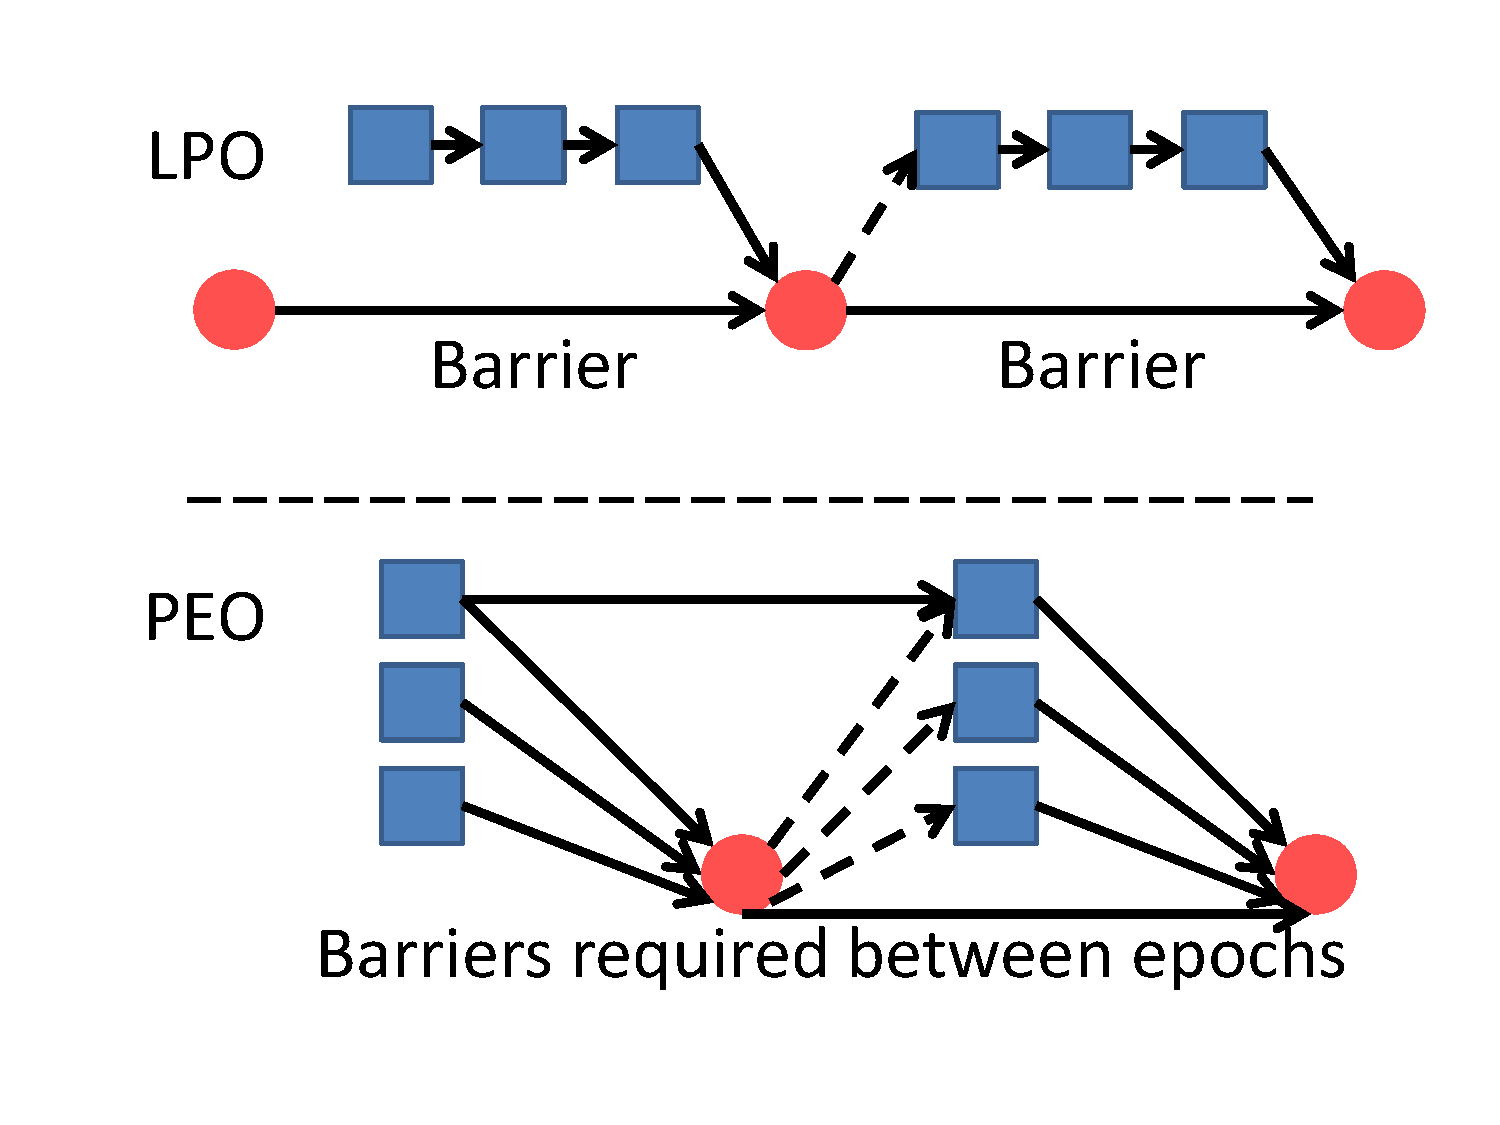
\includegraphics[width=.7\textwidth]{PMC_patterns/buffer_PEO_LPO.pdf}
\caption{\textbf{Buffer execution under LPO and PEO.}  LPO (top) removes persist dependencies between the counter value and subsequent buffer persists on other threads.  Dependencies remain when adjacent buffer inserts are from the same thread (dashed line).  PEO (bottom) allows buffer data to persist in parallel.}
\label{fig:buffer_PEO_LPO}
\end{figure}
